\documentclass[a4paper,11pt]{ujreport}
%%【PostScript, JPEG, PNG等の画像の貼り込み】
%% 利用するパッケージを選んでコメントアウトしてください.
\usepackage{graphicx} % for 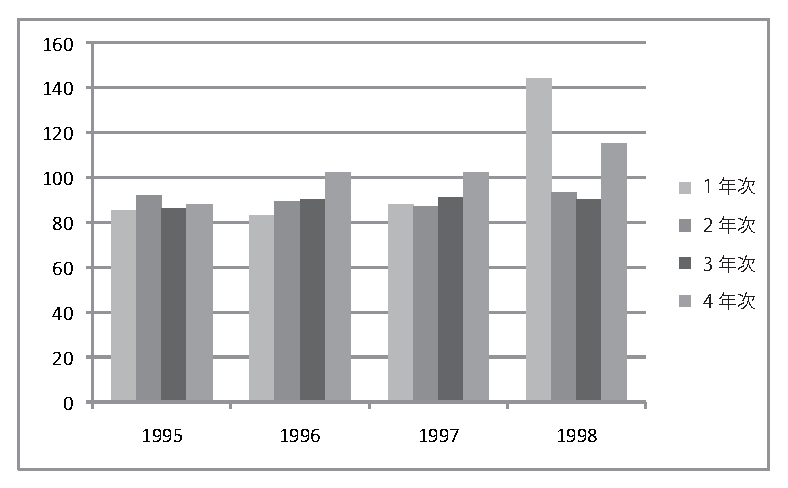
\includegraphics[width=3cm]{sample.eps}
\usepackage{epsfig} % for 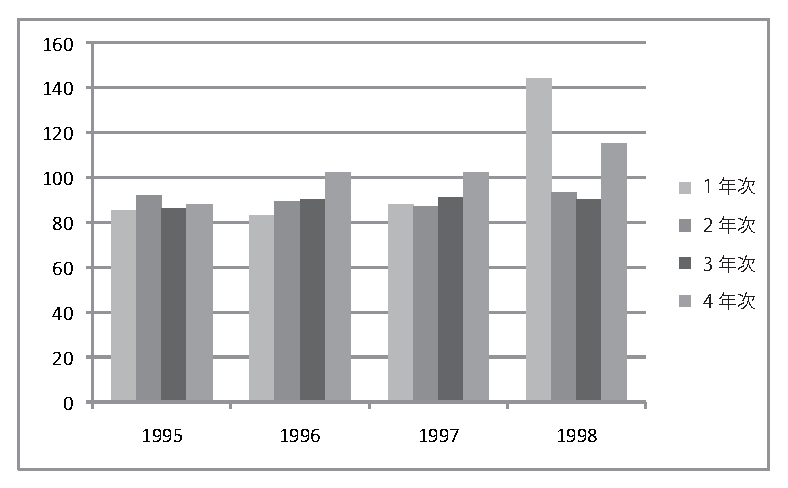
\psfig{file=sample.eps,width=3cm}
%\usepackage{epsf} % for \epsfile{file=sample.eps,scale=0.6}
%\usepackage{epsbox} % for \epsfile{file=sample.eps,scale=0.6}
\usepackage{/Users/takagihayata/workspace/materialize-mongodb/paper/mast/class/mediabb} % for pdf

\usepackage{times} % use Times Font instead of Computer Modern
% \usepackage{listings} % for soursecode
% \usepackage{plistings} % for soursecode
\usepackage{/Users/takagihayata/workspace/materialize-mongodb/paper/mast/class/docmute} % texファイル分割用

\setcounter{tocdepth}{3}
\setcounter{page}{-1}

\setlength{\oddsidemargin}{0.1in}
\setlength{\evensidemargin}{0.1in}
\setlength{\topmargin}{0in}
\setlength{\textwidth}{6in}
%\setlength{\textheight}{10.1in}
\setlength{\parskip}{0em}
\setlength{\topsep}{0em}

%\newcommand{\zu}[1]{{\gt \bf 図\ref{#1}}}

%% タイトル生成用パッケージ(重要)
\usepackage{/Users/takagihayata/workspace/materialize-mongodb/paper/mast/class/mast-jp-sjis}

%% タイトル
%% 【注意】タイトルの最後に\\ を入れるとエラーになります
\title{NoSQL型データベースシステムでの実体化ビュー選択に関する研究}
%% 著者
\author{髙木 颯汰}
%% 指導教員
\advisor{古瀬 一隆 陳 漢雄}

%% 年月 (提出年月)
%% 年月は必要に応じて書き替えてください.
\majorfield{ } \yearandmonth{2019年 1月}


\addtocounter{page}{2} %単体でコンパイルした際の調整用
\addtocounter{chapter}{2} %単体でコンパイルした際の調整用
\begin{document}

\chapter{提案手法}
\label{chap:ProposedAlgorithm}
\section{ドキュメント指向型データベースにおける実体化について}
\label{section:AboutMvInDocumentDB}
ドキュメント指向型データベースの特徴として埋め込み(embed)がある.従来のRDBでは複数の表による1対1や1対多,多対多の関係を表す際に,参照先のプライマリーキーのみを保存してSELECTされる際に結合処理を行う.それに対してドキュメント指向型データベースでは参照先の実データを参照元に埋め込むことができ,これによって結合処理を省くことができる.埋め込み先が複数の場合には更新処理が増加し,従来の参照型に比べてデータアクセスの柔軟性が損なわれるというデメリットがある\cite{Sky株式会社201212}.図\ref{figure:Reference}はドキュメント指向型データベースの参照型を,図\ref{figure:Embed}は図\ref{figure:Reference}のデータを埋込型で表した図である.

また.図\ref{figure:Reference}と図\ref{figure:Embed}のドキュメントを得るためのクエリを表\ref{table:MongoReferenceEmbedFind}に示す.参照型のクエリではMongoDBのaggregate(集計)メソッドを用いて参照先のドキュメントを結合している.まず,"\$match"演算子を用いてidが12345であるpeopleドキュメントをフィルタリングし,"\$lookup"演算子で参照先のドキュメントと結合している."\$lookup"演算子では参照先のコレクションを"from"で,参照元のidのフィールド名を"localField"で,参照先コレクション内でのidのフィールド名を"foreignField"で定義して結合処理を行なっている.埋込型のクエリではfamiliesドキュメントが埋め込まれているので,findメソッドを用いてidが12345であるpeopleドキュメントをフィルタリングし取得するだけで埋め込まれているfamiliesドキュメントも取得することができる.

idが123456のfamiliesドキュメントを更新するクエリを表\ref{table:MongoReferenceEmbedUpdate}に示す.両者ともMongoDBのupdateメソッドを用いている.第一引数には検索内容,第二引数には置き換えるドキュメントを指定している."\$set"演算子を用いることで第二引数で指定しているフィールド以外のデータを保持しつつ,更新処理を行うことができる.
参照型はfamiliesコレクションに対しての1度の更新処理だけで終了するが,埋込型に関しては埋め込まれているコレクション全てに対してクエリを実行する必要がある.
\begin{figure}[htbp]
	\begin{center}
		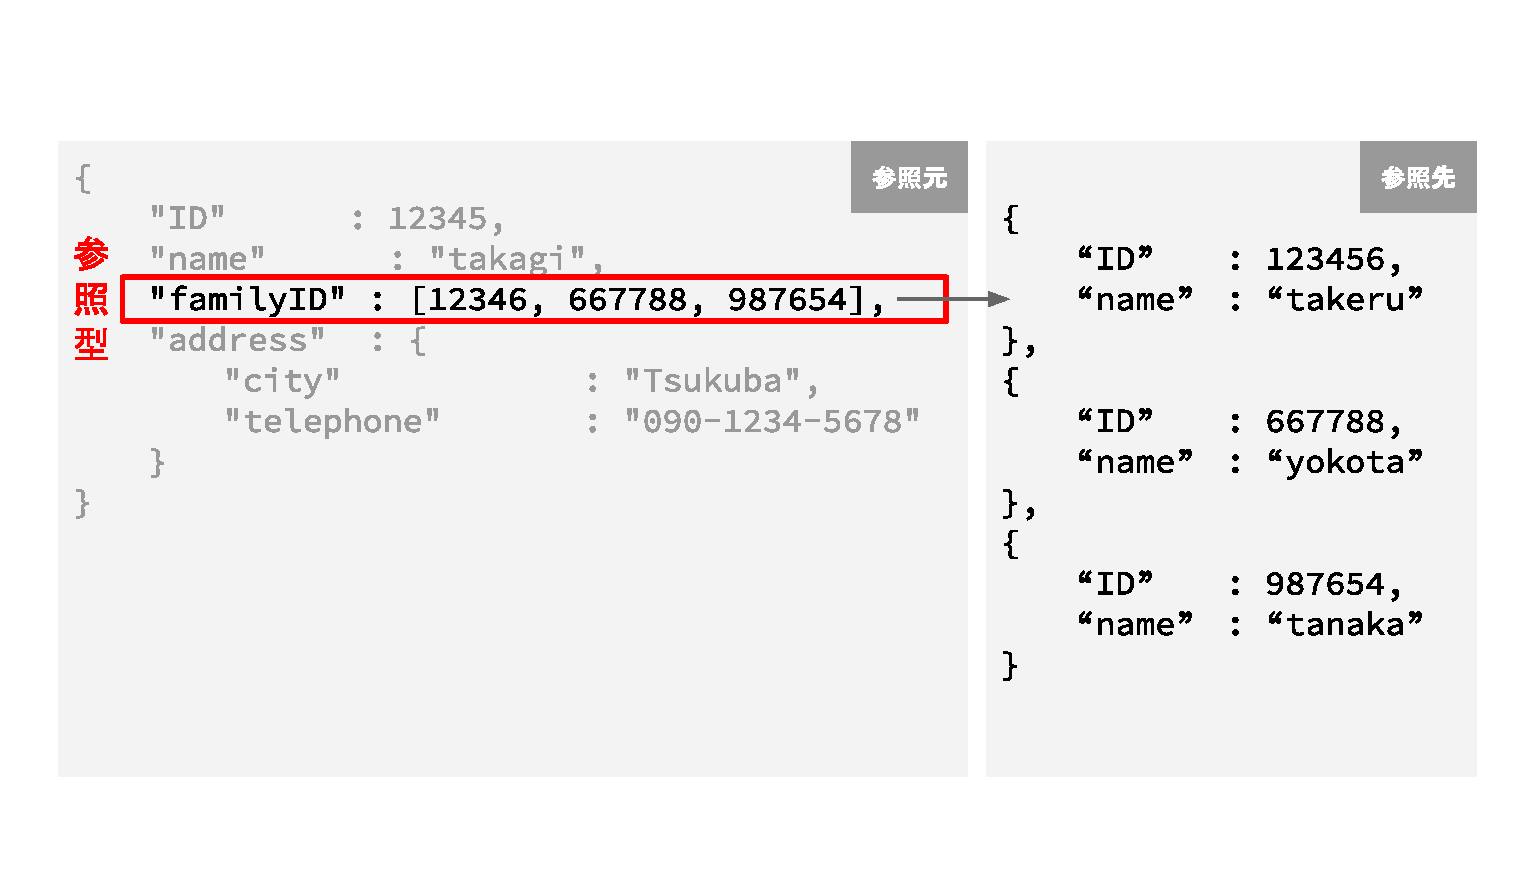
\includegraphics[width=30em, trim=0 5em 0 2em]{src/Reference.eps} %[trim=left bottom right top]
	\end{center}
	\caption{参照型}
	\label{figure:Reference}
\end{figure}
\begin{figure}[htbp]
	\begin{center}
		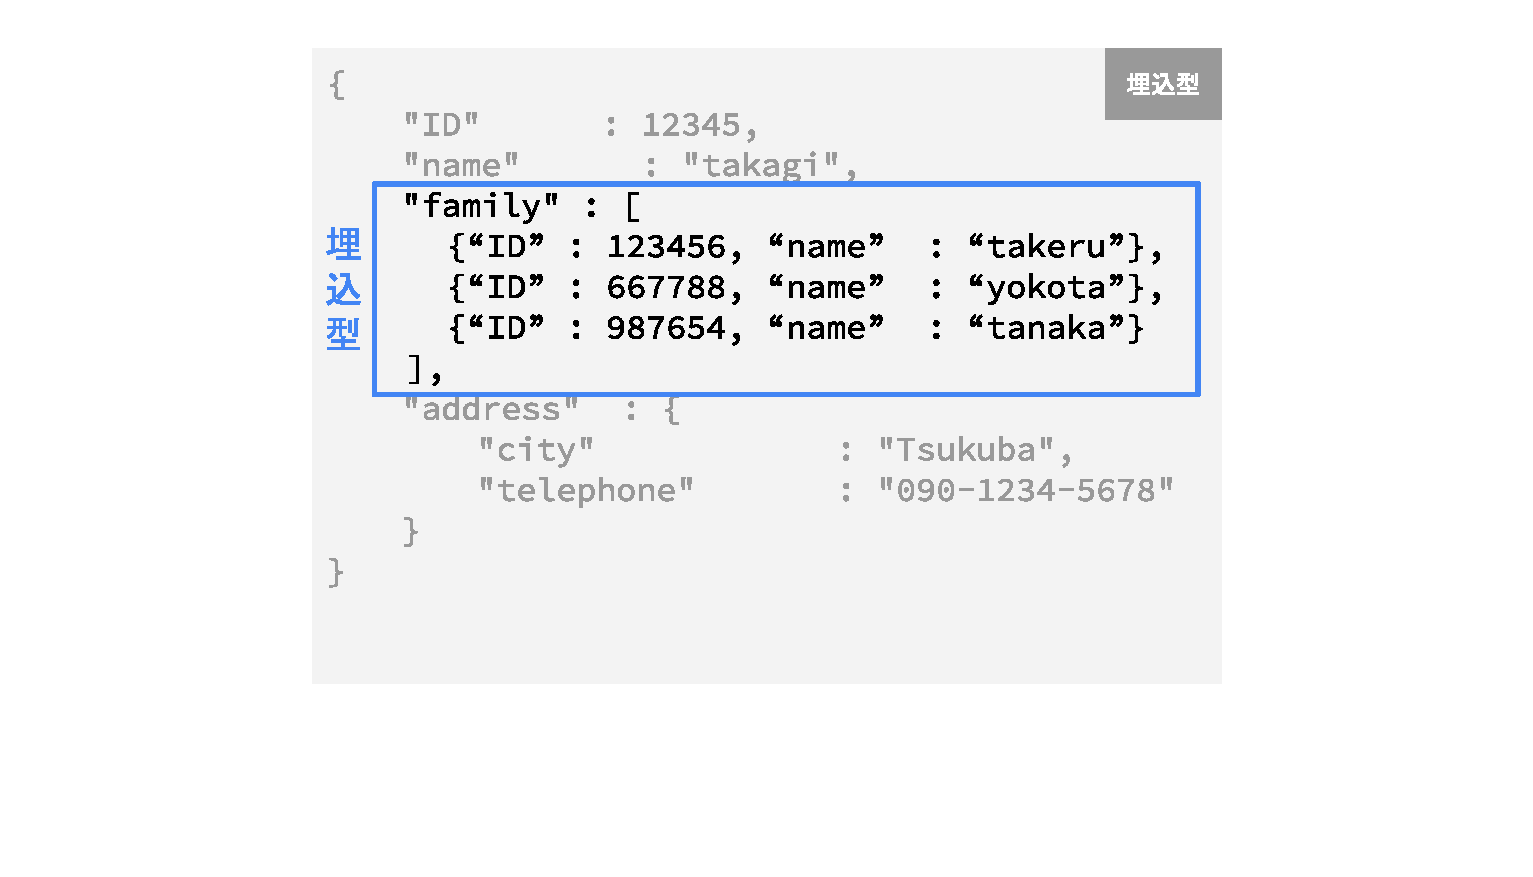
\includegraphics[width=30em, trim=0 7em 0 0em]{src/Embed.eps} %[trim=left bottom right top]
	\end{center}
	\caption{埋込型}
	\label{figure:Embed}
\end{figure}

\begin{table}[htb]
  \begin{center}
    \caption{MongoDBにおける参照型データモデルと埋込型データモデルでの検索クエリ}
		\label{table:MongoReferenceEmbedFind}
    \begin{tabular}{|c|l|} \hline
			参照型 &
			\begin{tabular}{l}
				db.people.aggregate([\\
				\ \ \{\$match: \{ID: 12345\}\},\\
				\ \ \{\$lookup: \{ from: "families", localField: "familyID", foreignField: "ID"\}\}\\
				]);
			\end{tabular}\\ \hline
			埋込型 &
			\begin{tabular}{l}
				db.people.find(\{ID: 12345\});
			\end{tabular}
			  \\ \hline
    \end{tabular}
  \end{center}
\end{table}
\begin{table}[htb]
  \begin{center}
    \caption{MongoDBにおける参照型データモデルと埋込型データモデルでの更新クエリ}
		\label{table:MongoReferenceEmbedUpdate}
    \begin{tabular}{|c|l|} \hline
			参照型 &
			\begin{tabular}{l}
				db.families.update(\{ ID: 123456\},\{ \$set: \{ name: "takebayashi"\}\});
			\end{tabular}\\ \hline
			埋込型 &
			\begin{tabular}{l}
				db.people.update(\{"family.ID": 12345\}, \{ \$set: \{family.\$.name: "takebayashi"\}\});
			\end{tabular}
			  \\ \hline
    \end{tabular}
  \end{center}
\end{table}

全てのドキュメントを埋め込み型として保存すると埋め込み先のドキュメントの更新処理が増え,著しく更新時間が増加する為,データモデルとして最適とは言えない.埋め込み型のデータモデルとして保存するコレクションを最適に選択し,データモデルを最適化することがドキュメント指向型データベースを高速に使用することに繋がる.本論文ではこの実体化するコレクションの選択を自動化する.

\section{提案手法の構成}
\label{section:ProposedAlgorithmArchitecture}
本論文ではドキュメント指向型データベースの埋込型データモデルをリレーショナルデータベースの実体化ビューと置き換えて考える.ドキュメント指向型データベースのよくアクセスされる部分や処理速度がネックとなっている部分を埋込型として別コレクションに保持することで“実体化ビュー作成”,どの部分を埋込型にするかの判断を“実体化ビュー選択”とする.図\ref{figure:ReferenceToEmbed}は本論文での“実体化ビュー作成”を示したものである.
\begin{figure}[htbp]
	\begin{center}
		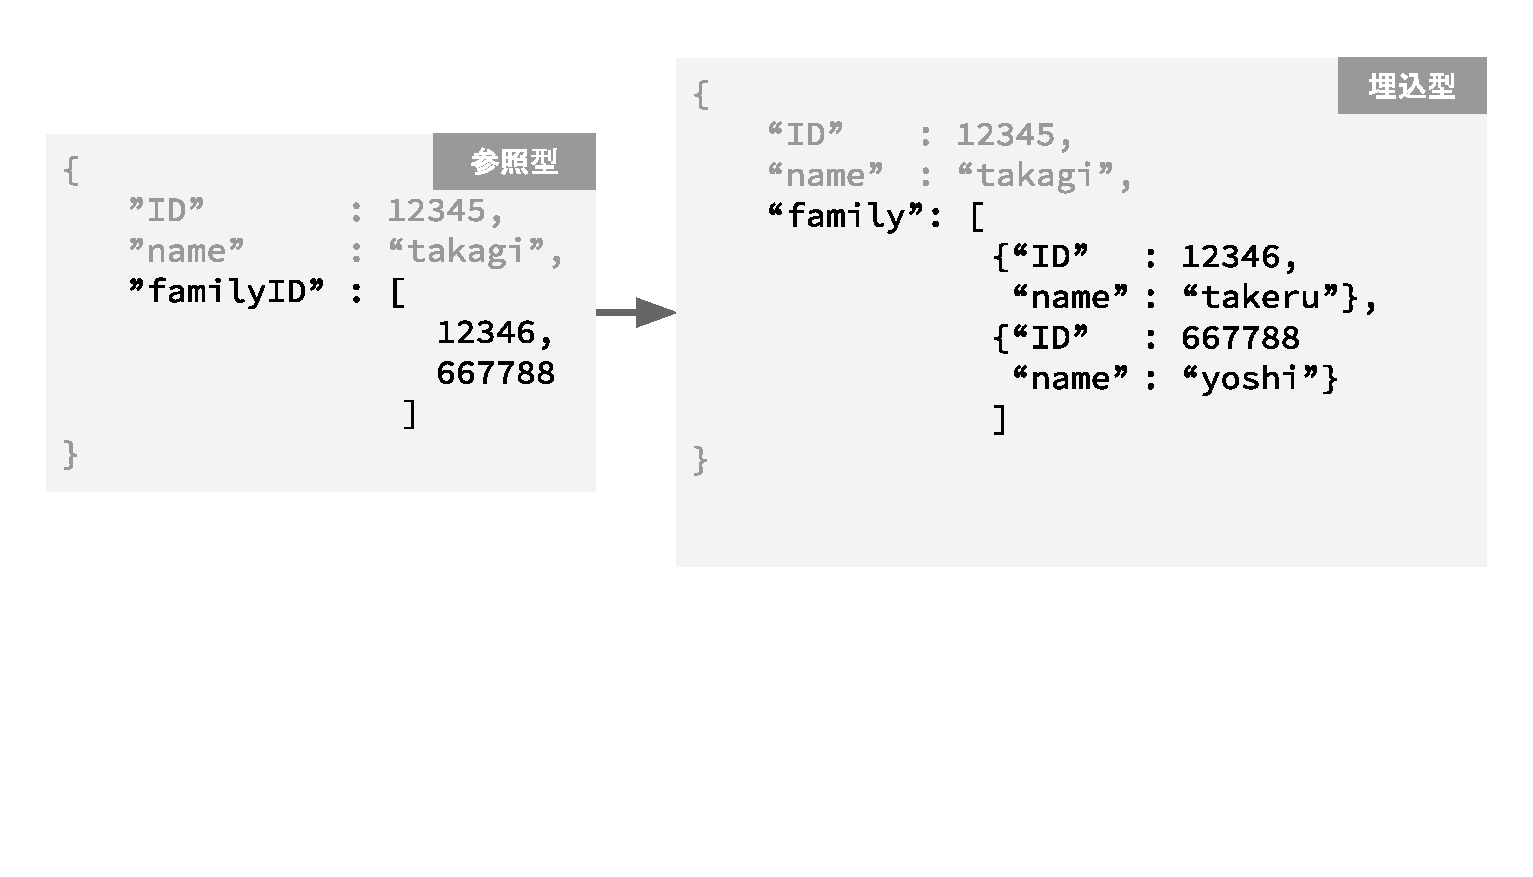
\includegraphics[width=30em, trim=0 13em 0 0]{src/ReferenceToEmbed.eps} %[trim=left bottom right top]
	\end{center}
	\caption{参照型から埋込型への書き換え}
	\label{figure:ReferenceToEmbed}
\end{figure}

実装システムについて図\ref{figure:Midleware}に示す.ユーザーからのデータアクセスから実体化ビュー作成までの流れを図\ref{figure:Midleware}を用いて説明する.
\begin{figure}[h]
	\begin{center}
		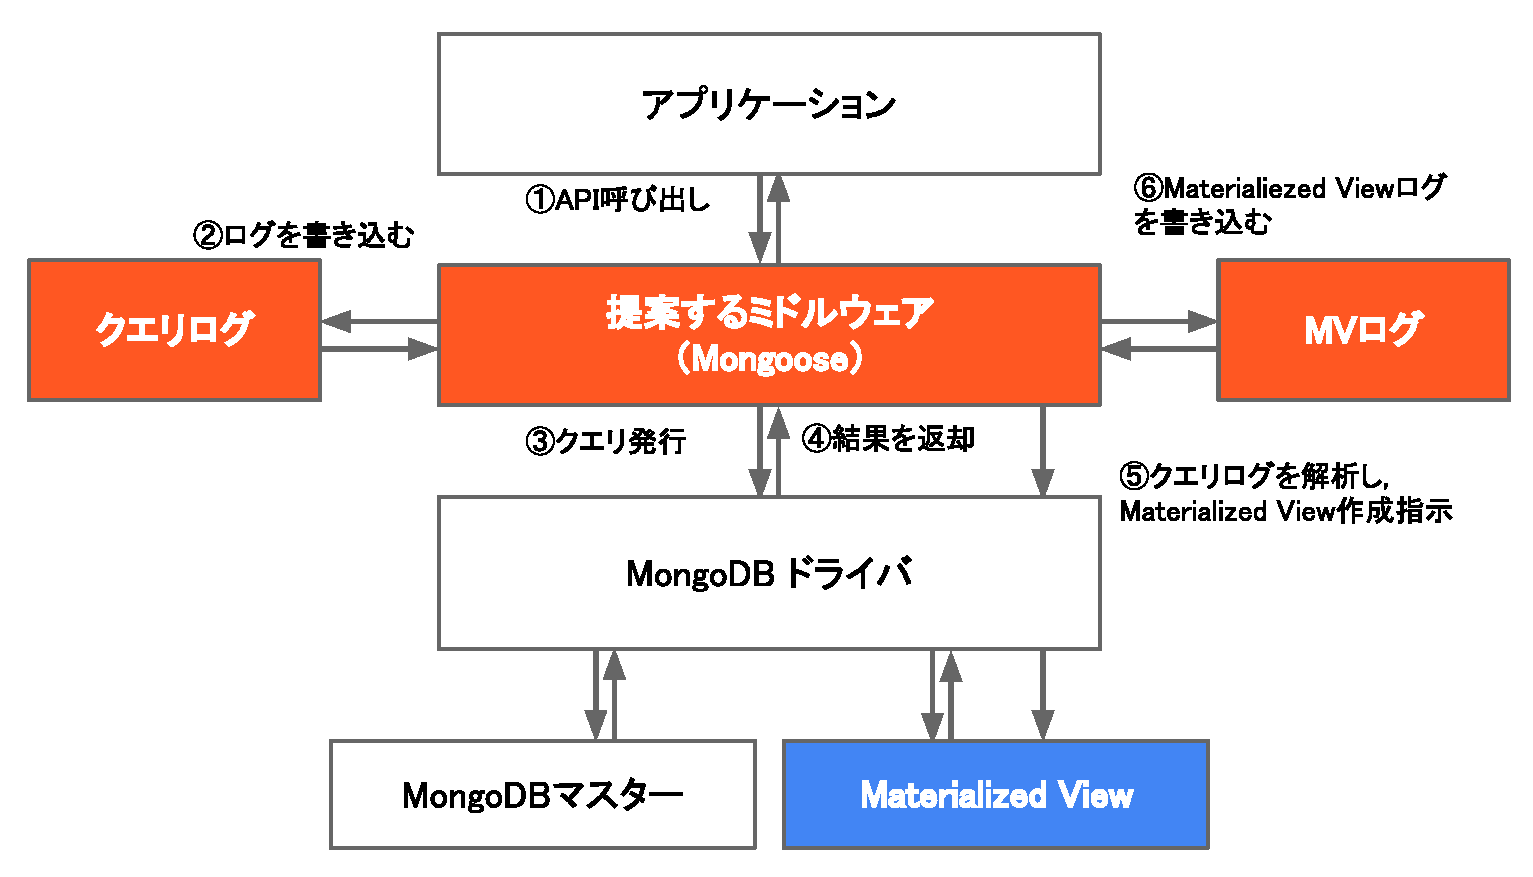
\includegraphics[width=30em]{src/Midleware.eps}
	\end{center}
	\caption{提案ミドルウェア(実体化前)}
	\label{figure:Midleware}
\end{figure}
図\ref{figure:Midleware}-①まずユーザーがアプリケーションからミドルウェアに対してデータアクセスの要求する.図\ref{figure:Midleware}-②ミドルウェアでは,頻繁にアクセスされるドキュメントを分析するために,クエリに関するログを残す.図\ref{figure:Midleware}-③次にMongoDBに対してクエリを発行する.図\ref{figure:Midleware}-④MongoDBから返ってきたクエリセットをアプリケーションに返却する.図\ref{figure:Midleware}-⑤クエリログを解析し,ボトルネックとなっているところや呼び出し回数の多い条件の実体化ビューを作成する.図\ref{figure:Midleware}-⑥実体化したドキュメントに関してログに記録する.

実体化した後のデータアクセスの流れを図\ref{figure:MidlewareMv}に示す.図\ref{figure:MidlewareMv}-①’アプリケーションからデータベースにアクセスがあった場合,まずログからアクセスされたデータが実体化されているか判定する.図\ref{figure:MidlewareMv}-②’実体化されている場合はクエリを書き換えて実体化ビューから結果を取得する.図\ref{figure:MidlewareMv}-③’アプリケーションに結果を返す際には元のクエリに合うように適宜変換する.
\begin{figure}[htbp]
	\begin{center}
		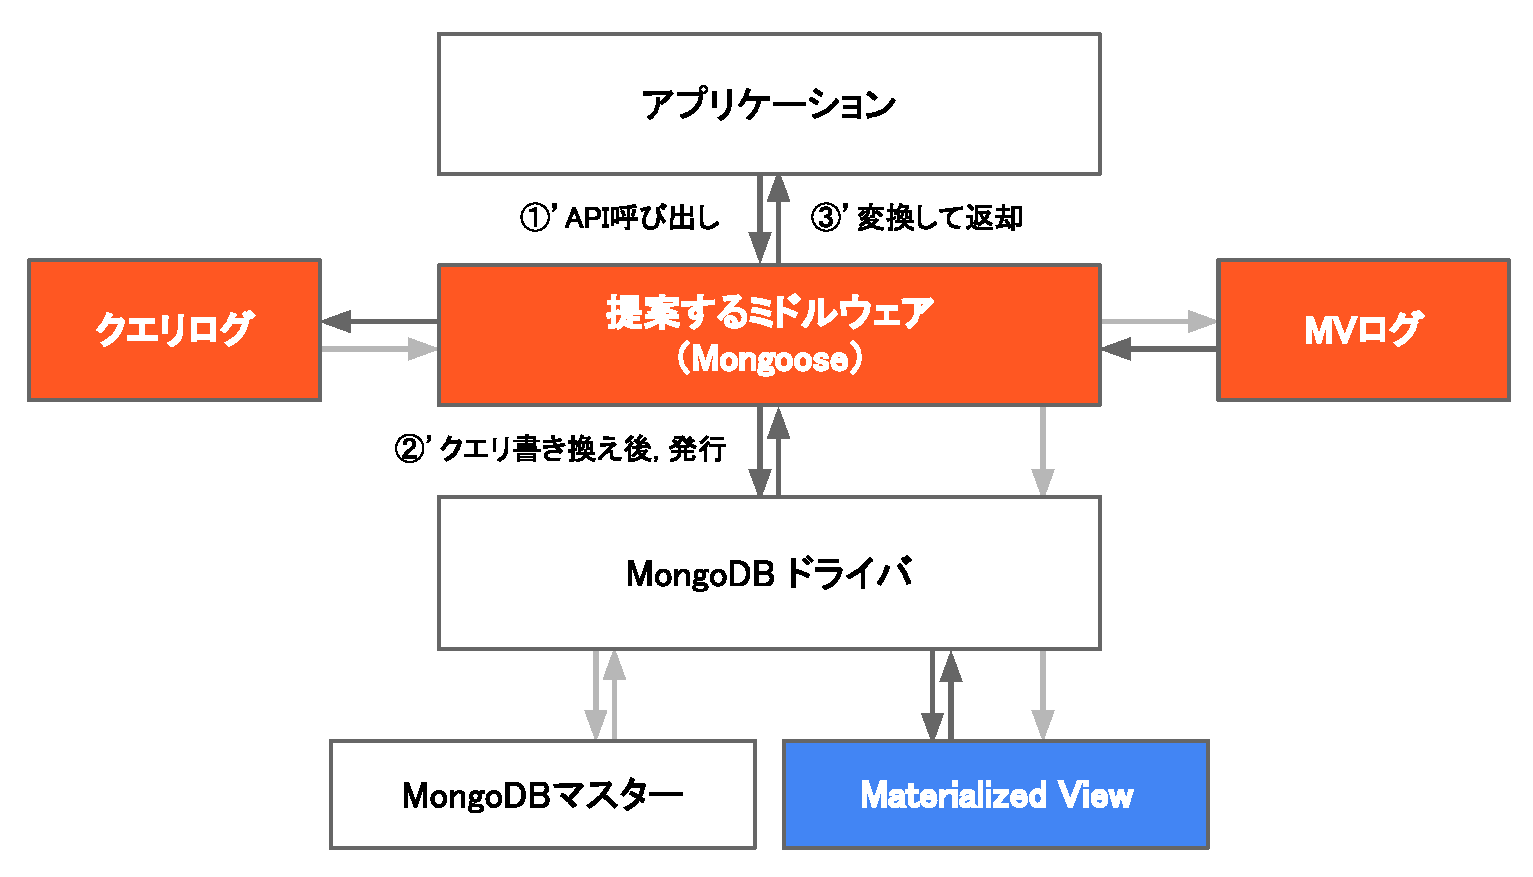
\includegraphics[width=30em]{src/MidlewareMv.eps} %[trim=left bottom right top]
	\end{center}
	\caption{提案ミドルウェア(実体化後)}
	\label{figure:MidlewareMv}
\end{figure}

次に具体的なクエリを用いて実装システムの流れを説明する.まだ実体化ビューが作成されていない,図\ref{figure:MidlewareExampleCollections}に示すようなpeopleコレクションとfamiliesコレクションに対して表\ref{table:MidlewareExampleQuery}のクエリが順に実行されたとする.クエリ1.1が実行された際にはまずMVログを確認し,peopleコレクションが実体化されているか確認する.実体化されていないので,クエリをそのままMongoDBのドライバに発行し,アプリケーションに結果を返す.その際にクエリログを記録する.各クエリに対するクエリログを表\ref{table:MidlewareExampleLog}に示す.クエリ1.2,1.3,1.4も同様にpeopleコレクションが実体化されていないので,そのままクエリが実行される.

\begin{figure}[htbp]
	\begin{center}
		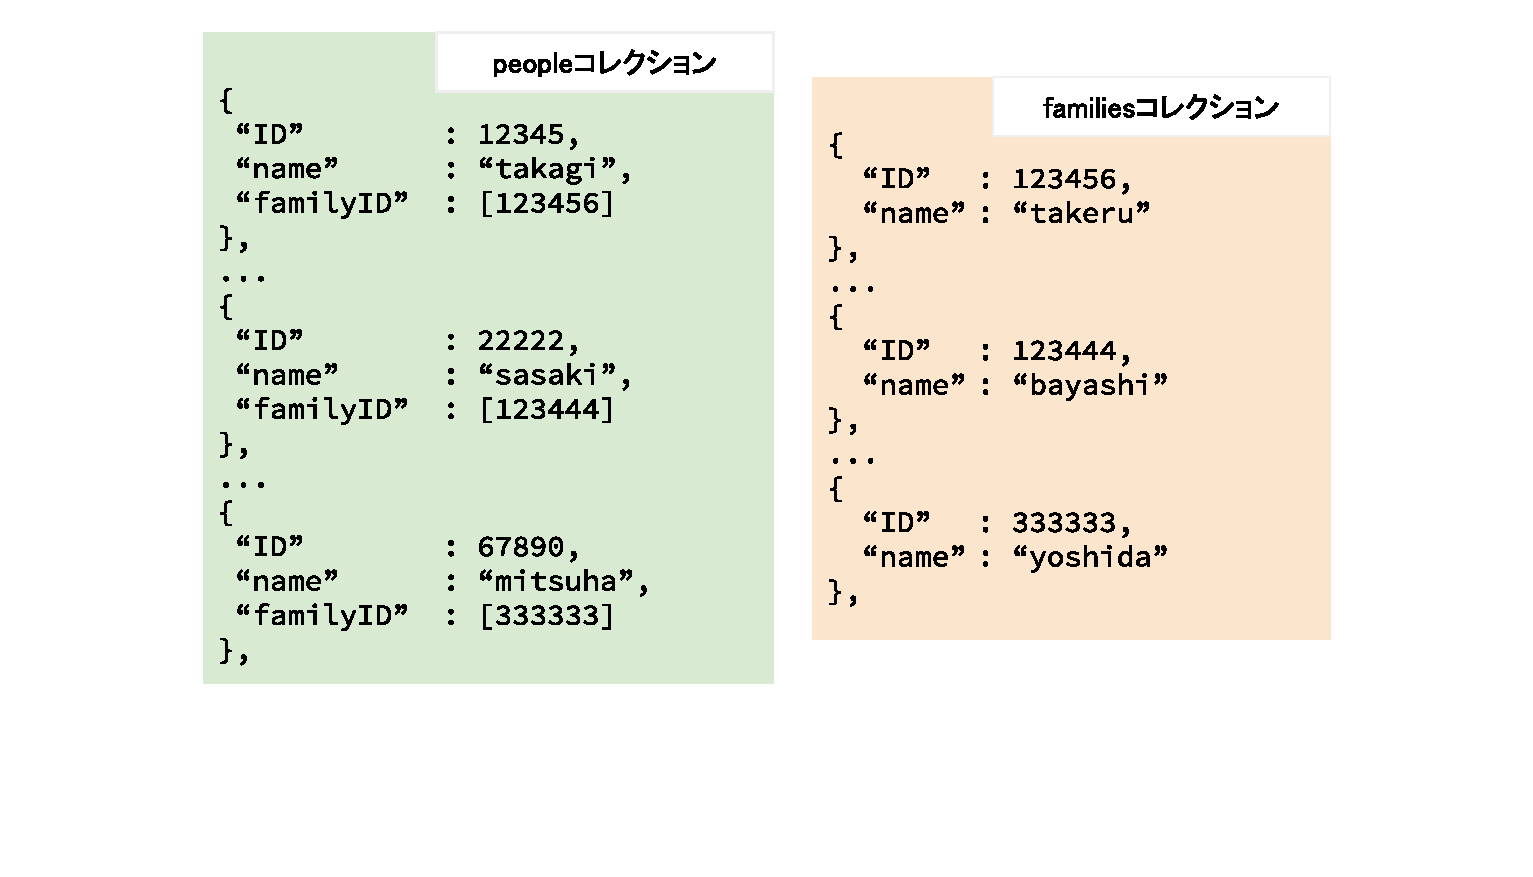
\includegraphics[width=30em, trim=0 10em 0 0]{src/MidlewareExampleCollections.eps} %[trim=left bottom right top]
	\end{center}
	\caption{peopleコレクションとfamilesコレクションの構成}
	\label{figure:MidlewareExampleCollections}
\end{figure}

\begin{table}[htb]
  \begin{center}
    \caption{ユーザークエリ1}
		\label{table:MidlewareExampleQuery}
    \begin{tabular}{|c|l|} \hline
			クエリ1.1 &
			\begin{tabular}{l}
				db.people.aggregate([\\
				\ \ \{\$match: \{ID: 12345\}\},\\
				\ \ \{\$lookup: \{ from: "families", localField: "familyID", foreignField: "ID"\}\}\\
				]);
			\end{tabular}\\ \hline
			クエリ1.2 &
			\begin{tabular}{l}
				db.people.aggregate([\\
				\ \ \{\$match: \{ID: 22222\}\},\\
				\ \ \{\$lookup: \{ from: "families", localField: "familyID", foreignField: "ID"\}\}\\
				]);
			\end{tabular}\\ \hline
			クエリ1.3 &
			\begin{tabular}{l}
				db.people.aggregate([\\
				\ \ \{\$match: \{ID: 67890\}\},\\
				\ \ \{\$lookup: \{ from: "families", localField: "familyID", foreignField: "ID"\}\}\\
				]);
			\end{tabular}\\ \hline
			クエリ1.4 &
			\begin{tabular}{l}
				db.families.update(\\
				\ \ \{ ID: 123456\},\\
				\ \ \{ \$set: \{ name: "takebayashi"\}\\
				\});
			\end{tabular}\\ \hline
    \end{tabular}
  \end{center}
\end{table}

\begin{table}[htb]
  \begin{center}
    \caption{ユーザークエリ1で記録されるクエリログ}
		\label{table:MidlewareExampleLog}
    \begin{tabular}{|c|l|} \hline
			クエリログ1.1 &
			\begin{tabular}{l}
				\{"method" : "aggregate",\\
				\ \ "lookup" : ["families"],\\
				\ \ "collection\_name" : "people",\\
				\ \ "query" : "\{\$match: \{ID: 12345\}\}",\\
				\ \ "elapsed\_time" : 55.66362400003709,\\
				\ \ "is\_rewrited" : false\}
			\end{tabular}\\ \hline
			クエリログ1.2 &
			\begin{tabular}{l}
				\{"method" : "aggregate",\\
				\ \ "lookup" : ["families"],\\
				\ \ "collection\_name" : "people",\\
				\ \ "query" : "\{\$match: \{ID: 22222\}\}",\\
				\ \ "elapsed\_time" : 42.66362400003732,\\
				\ \ "is\_rewrited" : false\}
			\end{tabular}\\ \hline
			クエリログ1.3 &
			\begin{tabular}{l}
				\{"method" : "aggregate",\\
				\ \ "lookup" : ["families"],\\
				\ \ "collection\_name" : "people",\\
				\ \ "query" : "\{\$match: \{ID: 67890\}\}",\\
				\ \ "elapsed\_time" : 57.26362400003767,\\
				\ \ "is\_rewrited" : false\}
			\end{tabular}\\ \hline
			クエリログ1.4 &
			\begin{tabular}{l}
				\{"method" : "update",\\
				\ \ "collection\_name" : "families",\\
				\ \ "query" : "\{ \$set: \{ name: "takebayashi"\}\}\}",\\
				\ \ "elapsed\_time" : 70.36362400003744,\\
				\ \ "is\_rewrited" : false\}
			\end{tabular}\\ \hline
    \end{tabular}
  \end{center}
\end{table}

クエリ1.4が実行された後に自動実体化のプロセス1が実行されたとする.実際の運用では集計やコレクションの作成などを行う可能性があるので,定期的にアクセスの少ない深夜帯などに実行されることが望ましい.このプロセス1では前述で記録したクエリログを元に実体化するコレクションを判定する.このプロセス1の詳細は\ref{section:MvAlgorithm}節で説明する.ここでは\ref{section:MvAlgorithm}節においてpeopleコレクションが実体化されたとする.その際に作成されたpeopleの実体化ビューのコレクション名を"mvpeople"とし,ドキュメントの内容を図\ref{figure:MidlewareExampleMV}に,同時に記録されるMVログを表\ref{table:MidlewareExampleMvLog}に示す.実体化したコレクション名を"original\_coll"で,参照先のコレクション名を"lookup"で,実体化ビューの削除フラグを"is\_deleted"で表している.

\begin{figure}[htbp]
	\begin{center}
		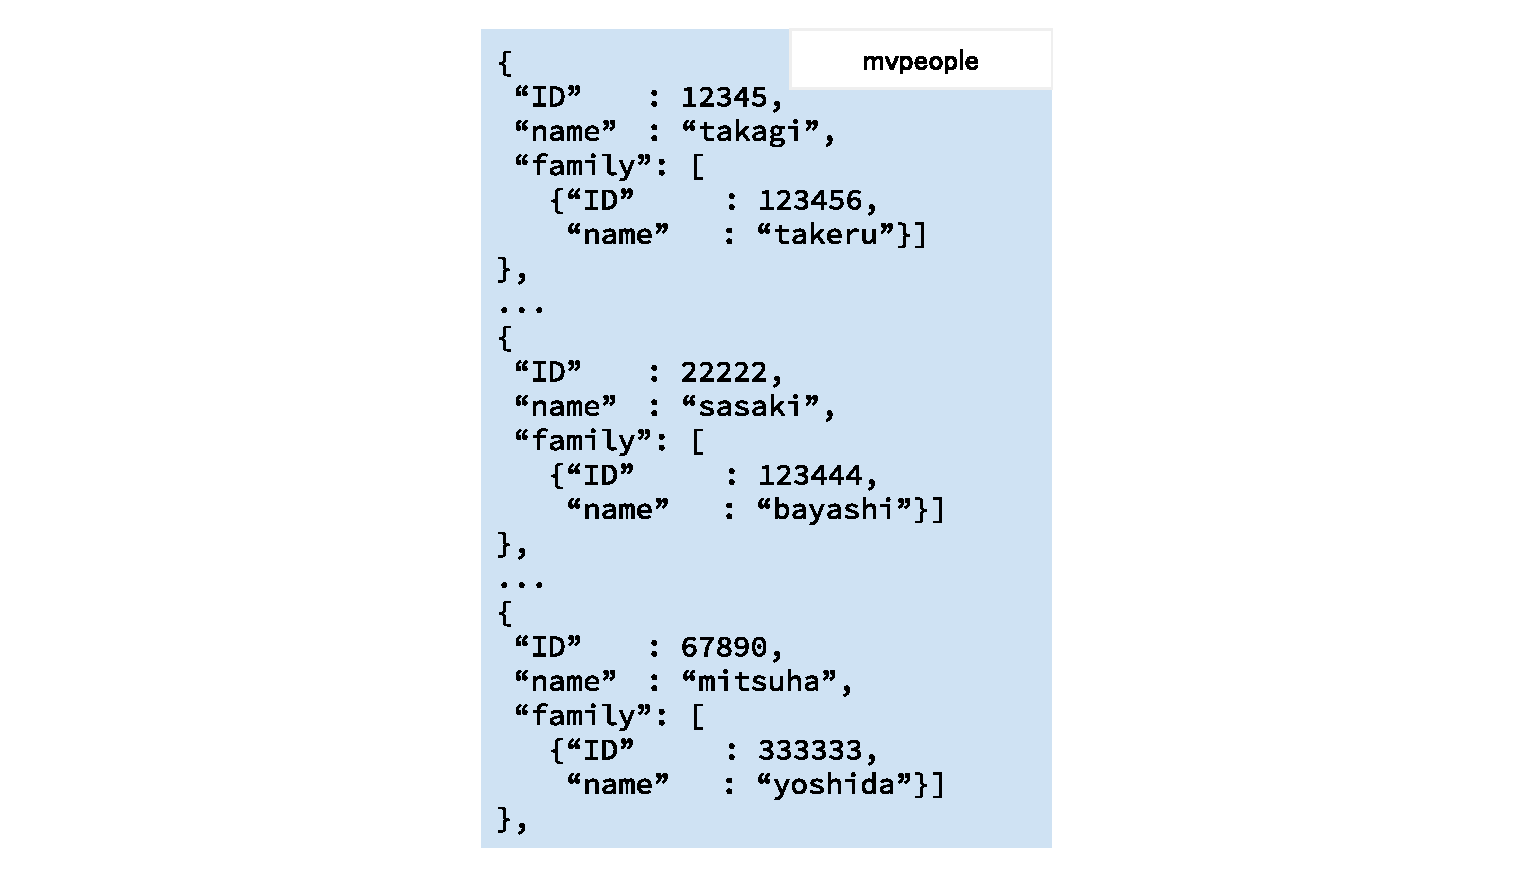
\includegraphics[width=30em, trim=0 0 0 0]{src/MidlewareExampleMV.eps} %[trim=left bottom right top]
	\end{center}
	\caption{peopleコレクションの実体化ビュー}
	\label{figure:MidlewareExampleMV}
\end{figure}

\begin{table}[htb]
  \begin{center}
    \caption{MVログ1}
		\label{table:MidlewareExampleMvLog}
    \begin{tabular}{|c|l|} \hline
			MVログ1 &
			\begin{tabular}{l}
				\{"original\_coll" : "people",\\
					\ \ "lookup" : [ "families" ],\\
					\ \ "is\_deleted" : false,
				\}
			\end{tabular}\\ \hline
    \end{tabular}
  \end{center}
\end{table}

次に表\ref{table:MidlewareExampleQuery2}のクエリが順に実行されたとする.クエリ2.1が実行された際にはまずMVログを取得し,peopleコレクションが実体化されているか確認する.表\ref{table:MidlewareExampleMvLog}から,peopleコレクションにfamiliesコレクションが埋め込まれた実体化ビューが存在するので,クエリを書き換えてMongoDBドライバにクエリを発行する.書き換え前と書き換え後のクエリの比較を表\ref{table:MidlewareExampleQueryRewrite}に示す.クエリ2.2ではfamiliesコレクションを更新しているが,表\ref{table:MidlewareExampleMvLog}からfamiliesドキュメントがpeopleコレクションに実体化ビューとして埋め込まれていることが分かるので,IDが123444のfamiliesドキュメントを保持しているpeopleドキュメントに関しても更新処理を行なっている.クエリ2.3ではpeopleコレクションの更新処理を行なっている.peopleコレクションは実体化されているので実体化ビューとオリジナルのコレクションの更新を同時に行う.

\begin{table}[htb]
  \begin{center}
    \caption{ユーザークエリ2}
		\label{table:MidlewareExampleQuery2}
		\begin{tabular}{|c|l|} \hline
			クエリ2.1 &
			\begin{tabular}{l}
				db.people.aggregate([\\
				\ \ \{\$match: \{ID: 67890\}\},\\
				\ \ \{\$lookup: \{\\
				\ \ \ \ \ from: "families",\\
				\ \ \ \ \ localField: "familyID",\\
				\ \ \ \ \ foreignField: "ID"\}\}\\
				]);
			\end{tabular}\\ \hline
			クエリ2.2 &
			\begin{tabular}{l}
				db.families.update(\\
				\ \ \{ ID: 123444\},\\
				\ \ \{ \$set: \{ name: "zenbayashi"\}\\
				\});
			\end{tabular}\\ \hline
			クエリ2.3 &
			\begin{tabular}{l}
				db.people.update(\\
				\ \ \{ ID: 12345\},\\
				\ \ \{ \$set: \{ name: "souta"\}\\
				\});
			\end{tabular}\\ \hline
    \end{tabular}
  \end{center}
\end{table}

\begin{table}[htb]
  \begin{center}
    \caption{書き換え後のユーザークエリ2}
		\label{table:MidlewareExampleQueryRewrite}
		\begin{tabular}{|c|l|l|} \hline
			 & \multicolumn{1}{|c|}{書き換え前のクエリ}
			 & \multicolumn{1}{|c|}{書き換え後のクエリ}
			 \\ \hline
			クエリ2.1 &
			\begin{tabular}{l}
				db.people.aggregate([\\
				\ \ \{\$match: \{ID: 67890\}\},\\
				\ \ \{\$lookup: \{\\
				\ \ \ \ \ from: "families",\\
				\ \ \ \ \ localField: "familyID",\\
				\ \ \ \ \ foreignField: "ID"\}\}\\
				]);
			\end{tabular} &
			\begin{tabular}{l}
				db.people.find([\\
				\ \ \{ID: 67890\}\\
				]);
			\end{tabular}\\ \hline
			クエリ2.2 &
			\begin{tabular}{l}
				db.families.update(\\
				\ \ \{ ID: 123444\},\\
				\ \ \{ \$set: \{ name: "zenbayashi"\}\\
				\});
			\end{tabular} &
			\begin{tabular}{l}
				db.families.update(\\
				\ \ \{ ID: 123444\},\\
				\ \ \{ \$set: \{ name: "zenbayashi"\}\\
				\});\\
				db.mvpeople.update(\\
				\ \ \{ family.ID: 123444\},\\
				\ \ \{ \$set: \{ family.\$.name: "zenbayashi"\}\\
				\});
			\end{tabular}\\ \hline
			クエリ2.3 &
			\begin{tabular}{l}
				db.people.update(\\
				\ \ \{ ID: 12345\},\\
				\ \ \{ \$set: \{ name: "souta"\}\\
				\});
			\end{tabular} &
			\begin{tabular}{l}
				db.mvpeople.update(\\
				\ \ \{ ID: 12345\},\\
				\ \ \{ \$set: \{ name: "souta"\}\\
				\});\\
				db.people.update(\\
				\ \ \{ ID: 12345\},\\
				\ \ \{ \$set: \{ name: "souta"\}\\
				\});
			\end{tabular}\\ \hline
    \end{tabular}
  \end{center}
\end{table}

\begin{table}[htb]
  \begin{center}
    \caption{ユーザークエリ2で記録されるクエリログ}
		\label{table:MidlewareExampleLog2}
    \begin{tabular}{|c|l|} \hline
			クエリログ2.1 &
			\begin{tabular}{l}
				\{"method" : "find",\\
				\ \ "collection\_name" : "people",\\
				\ \ "query" : "\{\$match: \{ID: 67890\}\}",\\
				\ \ "elapsed\_time" : 37.26362400003767,\\
				\ \ "is\_rewrited" : true\}
			\end{tabular}\\ \hline
			クエリログ2.2 &
			\begin{tabular}{l}
				\{"method" : "update",\\
				\ \ "collection\_name" : "families",\\
				\ \ "query" : "\{ \$set: \{ name: "zenbayashi"\}\}\}",\\
				\ \ "elapsed\_time" : 155.36362400003744,\\
				\ \ "is\_rewrited" : true\}\\
				\{"method" : "update",\\
				\ \ "collection\_name" : "people",\\
				\ \ "query" : "\{ \$set: \{ family.name: "zenbayashi"\}\}\}",\\
				\ \ "elapsed\_time" : 89.56362400003744,\\
				\ \ "is\_rewrited" : true\}
			\end{tabular}\\ \hline
			クエリログ2.3 &
			\begin{tabular}{l}
				\{"method" : "update",\\
				\ \ "collection\_name" : "people",\\
				\ \ "query" : "\{ \$set: \{ name: "souta"\}\}\}",\\
				\ \ "elapsed\_time" : 230.54762400003744,\\
				\ \ "is\_rewrited" : true\}
			\end{tabular}\\ \hline
    \end{tabular}
  \end{center}
\end{table}

クエリ2.3が実行された後に自動実体化のプロセス2が実行されたとする.実体化されているpeopleコレクションに対して逆実体化するべきか,実体化されていないfamiliesコレクションに対して実体化するべきかを評価する.逆実体化に関しては\ref{section:ReverseMvAlgorithm}節で詳しく説明する.ここでは\ref{section:ReverseMvAlgorithm}節でpeopleコレクションを逆実体化するべきだと判断されたとする.逆実体化時には該当のMVログに対して削除フラグを立てる.その際のMVログを表\ref{table:MidlewareExampleMvLog2}に示す.実体化時もオリジナルのコレクションに対して更新を行なっているので,逆実体化時にコレクションの操作は発生しない.

\begin{table}[htb]
  \begin{center}
    \caption{逆実体化後のMVログ}
		\label{table:MidlewareExampleMvLog2}
    \begin{tabular}{|c|l|} \hline
			MVログ &
			\begin{tabular}{l}
				\{"original\_coll" : "people",\\
					\ \ "lookup" : [ "families" ],\\
					\ \ "is\_deleted" : true,
				\}
			\end{tabular}\\ \hline
    \end{tabular}
  \end{center}
\end{table}

\section{実体化アルゴリズムについて}
\label{section:MvAlgorithm}
クエリログから実体化するコレクションを決定する条件を適切に設定することで,実体化ビュー選択を自動化することができる.この実体化条件については以下の条件が考えられる.
\begin{enumerate}
  \item クエリログの統計
  \item ドキュメント内の参照数
\end{enumerate}
1の条件は実際のクエリの検索回数・更新回数やその処理時間を元に実体化するコレクションを選定する.2の条件ではドキュメント内の他コレクションへの参照数を元に実体化後の更新処理の増加を予想し,実体化するコレクションを選定する.本論文では更新処理が用意であり,クエリに柔軟に対応できるクエリログの統計を元に実体化する条件を作成する.

\ref{section:ProposedAlgorithmArchitecture}節のプロセス1ではクエリログ1.1から1.4を集計して実体化するコレクションを決定する.提案手法では検索クエリ数と更新クエリ数の比があらかじめ決めた比を超えていた際に実体化を行う.クエリログ1.1から1.4を集計した結果を表\ref{table:MidlewareExampleAggregate1}に示す."is\_rewrited"でクエリが実体化ビューに対してか否かを,"total\_time"でクエリの合計処理時間を,"average\_time"でクエリの平均処理時間を,"count\_query"でクエリ数を表している.ここでは例として検索クエリ数/更新クエリ数比が20を超えていた際に実体化すると定義すると,プロセス1時点の検索クエリ数/更新クエリ数比はpeopleコレクションが3/0,familiesコレクションが0/1なので,peopleコレクションを実体化する.

\begin{table}[htb]
  \begin{center}
    \caption{プロセス1の際に取得されるクエリログ集計結果}
		\label{table:MidlewareExampleAggregate1}
    \begin{tabular}{|c|l|} \hline
			コレクション & \multicolumn{1}{|c|}{集計結果}\\\hline
			people &
			\begin{tabular}{l}
				\{ "\_id" : \{ "collection\_name" : "people",\\
				\ \ \ "method" : "findOne",\\
				\ \ \ "is\_rewrited" : false \},\\
				\ \ \ "total\_time" : 155.590872, \\
				\ \ \ "average\_time" : 51.863624,\\
				\ \ \ "count\_query" : 3 \}\\
			\end{tabular}\\ \hline
			families &
			\begin{tabular}{l}
				\{ "\_id" : \{ "collection\_name" : "families",\\
				\ \ \ "method" : "update",\\
				\ \ \ "is\_rewrited" : false \},\\
				\ \ \ "total\_time" : 70.36362400003744,\\
				\ \ \ "average\_time" : 70.36362400003744,\\
				\ \ \ "count\_query" : 1 \}\\
			\end{tabular}\\ \hline
    \end{tabular}
  \end{center}
\end{table}

\section{逆実体化アルゴリズムについて}
\label{section:ReverseMvAlgorithm}
クエリのログを元に実体化した場合,クエリの傾向が変わることで実体化していない状態の方が望ましくなる可能性や,コレクションの特性によっては実体化によるメリットがデメリットより少ない可能性がある.そのような事を防ぐために,定期的に実体化したコレクションに対してもメンテナンスを行い,場合によっては実体化したコレクションをオリジナルのデータモデルに戻すことが必要である.本論文では実体化したコレクションのデータモデルを元に戻す事を逆実体化と定義する.この逆実体化に対しても実体化同様,適切な逆実体化条件を設定する必要がある.

本論文ではクエリのログの統計から実体化後の検索処理時間と更新処理時間を比較し,各コレクションに対して逆実体化の必要性を確認する.

\ref{section:ProposedAlgorithmArchitecture}節のプロセス2では実体化されているコレクションのうち,クエリログ1.1から1.4とクエリログ2.1から2.3を集計して逆実体化するコレクションを決定する.クエリログ1.1から2.3を集計した結果を表\ref{table:MidlewareExampleAggregate2}に示す."is\_rewrited"が"true"であるオブジェクトが実体化後の集計結果である.peopleコレクションの実体化後の検索処理累計時間が37ms,更新処理累計時間が320msで,更新処理累計時間の方が長いので逆実体化を行う.

\begin{table}[htb]
  \begin{center}
    \caption{プロセス2の際に取得されるクエリログ集計結果}
		\label{table:MidlewareExampleAggregate2}
    \begin{tabular}{|c|l|} \hline
			コレクション & \multicolumn{1}{|c|}{集計結果}\\\hline
			people &
			\begin{tabular}{l}
				\{ "\_id" : \{ "collection\_name" : "people",\\
				\ \ \ "method" : "findOne",\\
				\ \ \ "is\_rewrited" : false \},\\
				\ \ \ "total\_time" : 155.590872, \\
				\ \ \ "average\_time" : 51.863624,\\
				\ \ \ "count\_query" : 3 \}\\

				\{ "\_id" : \{ "collection\_name" : "people",\\
				\ \ \ "method" : "findOne",\\
				\ \ \ "is\_rewrited" : true \},\\
				\ \ \ "total\_time" : 37.263624,\\
				\ \ \ "average\_time" : 37.263624,\\
				\ \ \ "count\_query" : 1 \}\\

				\{ "\_id" : \{ "collection\_name" : "people",\\
				\ \ \ "method" : "update",\\
				\ \ \ "is\_rewrited" : true \},\\
				\ \ \ "total\_time" : 320.111248,\\
				\ \ \ "average\_time" : 160.055624,\\
				\ \ \ "count\_query" : 2 \}\\
			\end{tabular}\\ \hline
			families &
			\begin{tabular}{l}
				\{ "\_id" : \{ "collection\_name" : "families",\\
				\ \ \ "method" : "update",\\
				\ \ \ "is\_rewrited" : false \},\\
				\ \ \ "total\_time" : 225.727248,\\
				\ \ \ "average\_time" : 112.863624,\\
				\ \ \ "count\_query" : 2 \}\\
			\end{tabular}\\ \hline
    \end{tabular}
  \end{center}
\end{table}

\end{document}
